\chapter{Analiza wyników}


\section{Ocena jakości różnych architektur sieci neuronowych}

\begin{table}
    \caption{Porównanie jakości predykcji różnych architektur splotowych sieci neuronowych}
    \begin{center}
        \begin{tabular}{|l|l|l|l|l|}
            \hline
            Architektura             & Liczba parametrów & F1             & Wykresy funkcji błędu i F1     & Macierz pomyłek                     \\
            \hline
            EfficientNet B0          & 5.3M             & 0.860          & rys. \ref{fig:plot_efficientnet_b0} & rys. \ref{fig:confusion_efficientnet_b0} \\
            \hline
            EfficientNet B1          & 7.8M             & 0.850          & rys. \ref{fig:plot_efficientnet_b1} & rys. \ref{fig:confusion_efficientnet_b1} \\
            \hline
            EfficientNet B2          & 9.2M             & 0.860          & rys. \ref{fig:plot_efficientnet_b2} & rys. \ref{fig:confusion_efficientnet_b2} \\
            \hline
            EfficientNet B3          & 12.0M            & 0.870          & rys. \ref{fig:plot_efficientnet_b3} & rys. \ref{fig:confusion_efficientnet_b3} \\
            \hline
            \textbf{EfficientNet B4} & \textbf{19.0M}   & \textbf{0.880} & rys. \ref{fig:plot_efficientnet_b4} & rys. \ref{fig:confusion_efficientnet_b4} \\
            \hline
            EfficientNet B5          & 30.0M            & 0.860          & rys. \ref{fig:plot_efficientnet_b5} & rys. \ref{fig:confusion_efficientnet_b5} \\
            \hline
            DenseNet121              & 8.0M             & 0.850          & rys. \ref{fig:plot_densenet121}     & rys. \ref{fig:confusion_densenet121}     \\
            \hline
            DenseNet169              & 14.1M            & 0.840          & rys. \ref{fig:plot_densenet169}     & rys. \ref{fig:confusion_densenet169}     \\
            \hline
            DenseNet201              & 20.0M            & 0.850          & rys. \ref{fig:plot_densenet201}     & rys. \ref{fig:confusion_densenet201}     \\
            \hline
            ResNet18                 & 11.7M            & 0.840          & rys. \ref{fig:plot_resnet18}        & rys. \ref{fig:confusion_resnet18}        \\
            \hline
        \end{tabular}
    \end{center}
    \label{tab:comparison}
\end{table}
\begin{table}
    \caption{Podsumowanie miary F1 dla poszczególnych klas (EfficientNet B4)}
    \begin{center}
        \begin{tabular}{|l|l|l|l|l|}
            \hline
            Klasa & Precyzja & Czułość & F1    & Liczba próbek \\
            \hline
            BLA   & 0.780    & 0.840   & 0.810 & 2311          \\
            \hline
            EBO   & 0.940    & 0.960   & 0.950 & 5532          \\
            \hline
            EOS   & 0.980    & 0.980   & 0.980 & 1192          \\
            \hline
            LYT   & 0.910    & 0.930   & 0.920 & 5193          \\
            \hline
            MON   & 0.720    & 0.730   & 0.720 & 825           \\
            \hline
            MYB   & 0.780    & 0.660   & 0.710 & 1323          \\
            \hline
            NGB   & 0.780    & 0.790   & 0.790 & 1962          \\
            \hline
            NGS   & 0.930    & 0.930   & 0.930 & 5984          \\
            \hline
            PEB   & 0.780    & 0.650   & 0.710 & 552           \\
            \hline
            PLM   & 0.940    & 0.860   & 0.900 & 1466          \\
            \hline
            PMO   & 0.830    & 0.840   & 0.840 & 2429          \\
            \hline
        \end{tabular}
    \end{center}
    \label{tab:f1_summary}
\end{table}

Niniejszy projekt ma za zadanie porównać różne architektury splotowych sieci neuronowych i wskazać, która z nich daje najlepsze rezultaty.
Tabela~\ref{tab:comparison} przedstawia porównanie wyników F1 dla poszczególnych eksperymentów.
Dla każdej architektury wskazano jej wielkość (ilość parametrów trenowalnych) oraz ważony wynik F1.
Większy wynik F1 informuje o lepszym zachowaniu modelu w rozpoznawaniu typów komórek.

Warto zauważyć, że \textcolor{red}{często wielkość sieci neuronowej (liczba wag)} \textcolor{red}{nie jest liniowo zależna} z jakością uzyskiwanych predykcji.
Dzieje się tak ze względu na to, że pojemność zachowania informacji nawet w mniejszej sieci jest wystarczająca, by móc rozpoznawać rodzaje komórek.

\begin{figure}
    \centering
    \includegraphics[width=\textwidth]{experiments/efficientnet_b0/combined}
    \caption{Wykres zależności funkcji straty i F1 od epoki trenowania (EfficientNet B0)}
    \label{fig:plot_efficientnet_b0}
\end{figure}
\begin{figure}
    \centering
    \includegraphics[width=0.8\textwidth]{experiments/efficientnet_b0/confusion_matrix}
    \caption{Macierz pomyłek modelu EfficientNet B0}
    \label{fig:confusion_efficientnet_b0}
\end{figure}

\begin{figure}
    \centering
    \includegraphics[width=\textwidth]{experiments/efficientnet_b1/combined}
    \caption{Wykres zależności funkcji straty i F1 od epoki trenowania (EfficientNet B1)}
    \label{fig:plot_efficientnet_b1}
\end{figure}
\begin{figure}
    \centering
    \includegraphics[width=0.8\textwidth]{experiments/efficientnet_b1/confusion_matrix}
    \caption{Macierz pomyłek modelu EfficientNet B1}
    \label{fig:confusion_efficientnet_b1}
\end{figure}

\begin{figure}
    \centering
    \includegraphics[width=\textwidth]{experiments/efficientnet_b2/combined}
    \caption{Wykres zależności funkcji straty i F1 od epoki trenowania (EfficientNet B2)}
    \label{fig:plot_efficientnet_b2}
\end{figure}
\begin{figure}
    \centering
    \includegraphics[width=0.8\textwidth]{experiments/efficientnet_b2/confusion_matrix}
    \caption{Macierz pomyłek modelu EfficientNet B2}
    \label{fig:confusion_efficientnet_b2}
\end{figure}

\begin{figure}
    \centering
    \includegraphics[width=\textwidth]{experiments/efficientnet_b3/combined}
    \caption{Wykres zależności funkcji straty i F1 od epoki trenowania (EfficientNet B3)}
    \label{fig:plot_efficientnet_b3}
\end{figure}
\begin{figure}
    \centering
    \includegraphics[width=0.8\textwidth]{experiments/efficientnet_b3/confusion_matrix}
    \caption{Macierz pomyłek modelu EfficientNet B3}
    \label{fig:confusion_efficientnet_b3}
\end{figure}

\begin{figure}
    \centering
    \includegraphics[width=\textwidth]{experiments/efficientnet_b4/combined}
    \caption{Wykres zależności funkcji straty i F1 od epoki trenowania (EfficientNet B4)}
    \label{fig:plot_efficientnet_b4}
\end{figure}
\begin{figure}
    \centering
    \includegraphics[width=0.8\textwidth]{experiments/efficientnet_b4/confusion_matrix}
    \caption{Macierz pomyłek modelu EfficientNet B4}
    \label{fig:confusion_efficientnet_b4}
\end{figure}

\begin{figure}
    \centering
    \includegraphics[width=\textwidth]{experiments/efficientnet_b5/combined}
    \caption{Wykres zależności funkcji straty i F1 od epoki trenowania (EfficientNet B5)}
    \label{fig:plot_efficientnet_b5}
\end{figure}
\begin{figure}
    \centering
    \includegraphics[width=0.8\textwidth]{experiments/efficientnet_b5/confusion_matrix}
    \caption{Macierz pomyłek modelu EfficientNet B5}
    \label{fig:confusion_efficientnet_b5}
\end{figure}

\begin{figure}
    \centering
    \includegraphics[width=\textwidth]{experiments/densenet121/combined}
    \caption{Wykres zależności funkcji straty i F1 od epoki trenowania (DenseNet121)}
    \label{fig:plot_densenet121}
\end{figure}
\begin{figure}
    \centering
    \includegraphics[width=0.8\textwidth]{experiments/densenet121/confusion_matrix}
    \caption{Macierz pomyłek modelu DenseNet121}
    \label{fig:confusion_densenet121}
\end{figure}

\begin{figure}
    \centering
    \includegraphics[width=\textwidth]{experiments/densenet169/combined}
    \caption{Wykres zależności funkcji straty i F1 od epoki trenowania (DenseNet169)}
    \label{fig:plot_densenet169}
\end{figure}
\begin{figure}
    \centering
    \includegraphics[width=0.8\textwidth]{experiments/densenet169/confusion_matrix}
    \caption{Macierz pomyłek modelu DenseNet169}
    \label{fig:confusion_densenet169}
\end{figure}

\begin{figure}
    \centering
    \includegraphics[width=\textwidth]{experiments/densenet201/combined}
    \caption{Wykres zależności funkcji straty i F1 od epoki trenowania (DenseNet201)}
    \label{fig:plot_densenet201}
\end{figure}
\begin{figure}
    \centering
    \includegraphics[width=0.8\textwidth]{experiments/densenet201/confusion_matrix}
    \caption{Macierz pomyłek modelu DenseNet201}
    \label{fig:confusion_densenet201}
\end{figure}

\begin{figure}
    \centering
    \includegraphics[width=\textwidth]{experiments/resnet18/combined}
    \caption{Wykres zależności funkcji straty i F1 od epoki trenowania (ResNet18)}
    \label{fig:plot_resnet18}
\end{figure}
\begin{figure}
    \centering
    \includegraphics[width=0.8\textwidth]{experiments/resnet18/confusion_matrix}
    \caption{Macierz pomyłek modelu ResNet18}
    \label{fig:confusion_resnet18}
\end{figure}


%TODO net
Najlepsze wyniki uzyskuje model używający architektury \textit{EfficientNet B4}.
Ważony wynik F1 w jej przypadku wynosi \textit{0.88}.
Tabela ~\ref{tab:f1_summary} przedstawia zestawienie precyzji, czułości i F1 dla poszczególnych klas.
Z kolei wykresy na rys. \ref{fig:plot_efficientnet_b4} przedstawiają zależności funkcji straty i F1 od epoki trenowania.
Można stwierdzić, że jakość modelu nie poprawia się znacząco wraz z kolejnymi iteracjami.
Macierz pomyłek jest widoczna natomiast na rys. \ref{fig:confusion_efficientnet_b4}.
Informuje ona, które klasy są najczęściej mylone między sobą.

\textcolor{red}{
Na podstawie wykresów funkcji straty i F1, można stwierdzić, że dla wszystkich sieci neuronowych już pierwsza epoka skutkowała rozpoznaniem wzorców.
Kolejne epoki nie poprawiały \textcolor{green}{drastycznie} skuteczności sieci.
Często mylonymi komórkami były promielocyty (\textit{PMO}) i mielocyty (\textit{MYB}), wynika to z tego, że ich wygląd jest podobny.
}

\section{Porównanie z innymi algorytmami}

\begin{figure}
    \centering
    \includegraphics[width=0.6\textwidth]{resnext_confusion_matrix}
    \caption{Macierz pomyłek dla modelu ResNeXt \cite{resnext}}
    \label{fig:resnext_confusion_matrix}
\end{figure}

Dostawca zbioru danych, w artykule \textit{Highly accurate differentiation of bone marrow cell morphologies using deep neural networks on a large image dataset} \cite{resnext} wykorzystuje architekturę \textit{ResNetXt-50}.
Model zawierający ponad 23 miliony parametrów był trenowany na \textit{NVIDIA TESLA V100} przez ok. 48 godzin.
Podobnie jak w niniejszym projekcie, autorzy artykułu wykonali normalizację intensywności kolorów przed trenowaniem sieci neuronowej (z powodu różnic w barwieniu Maya-Grünwalda-Giemsa).
Uzyskany ważony wynik F1 dla architektury \textit{ResNeXt-50} wyniósł \textit{0.822}.
Macierz pomyłek dostarczona przed autorów pracy jest widoczna na rys. \ref{fig:resnext_confusion_matrix}.


\section{Wyzwania}

Głównym wyzwaniem w trakcie realizacji projektu było wytrenowanie dużych sieci neuronowych.
Niestety, ich trening na lokalnym sprzęcie takim jak komputer osobisty jest bardzo czasochłonny.
W związku z tym konieczne było uruchamianie ich na platformie \textit{kaggle.com}, która oferuje 30 godzin czasu procesora graficznego miesięcznie.
Nieodpłatna możliwość pracy na platformie pozwoliła na pomyślną realizację projektu.


\section{Wnioski}

%TODO net
Zaprezentowane porównanie różnych splotowych sieci neuronowych pokazuje, że najlepszym modelem do zadania klasyfikacji rodzajów komórek w szpiku kostnym jest \textit{EfficientNet B4}.
Wybrana sieć neuronowa uzyskuje najlepszy ważony wynik F1 równy \textit{0.88}.
Warto też zwrócić uwagę na to, że sieci neuronowe znacznie większe od \textit{EfficientNet B4} nie dawały dużo lepszych rezultatów.

